\chapter{Networking}
The two key aspects of a network are:
\begin{enumerate}
   \item \textbf{Bandwidth} $\longrightarrow$ amount of data per second that can be moved through a specific connection
   \item \textbf{Latency} $\longrightarrow$ is the amount of time required for trasmitting data, measured from the moment it is sent from the source to the one it is available to the source.
\end{enumerate}
Latency ---in a datacenter--- to transmit data on the cable using \textit{``pure ethernet''} is of the order of $0.5\times10^{-6}s (\mu s)$.\\
If the TCP/IP stack is used (standard application case), latency is about $70-90\mu s$.

Furthermore, current drives have reached speeds such that latency may act as bottleneck between them and the CPU.

Cable aggregation (e.g. aggregating 4 cables 10Gbit/s, providing 40Gbit/s total)can be performed only at a low ---physical--- level. Otherwise the TCP/IP stream will be associated to a single cable of the ones aggregated, resulting in less bandwidth.
\framedt{Latency-sensitive}
{
   Some workloads are called \textit{latency-sensitive}, making the latency introduced by TCP-IP stack a problem.\\
   Inside a datacenter nowadays the typical latency is sub microsecond.
   
   Regarding this issue, technologies mentioned earlier come in handy; 
   \textit{InfiniBand} is a fabric technology that allows to have a very low latency, and is used in HPC\footnote{High performance computing} environments, and \textit{OmniPath} is a technology that is similar to InfiniBand, but is more scalable and is its natural successor.
   Also \textit{RDMA} and \textit{RoCE} are technologies that allow to access memory of a remote machine without involving the CPU or the OS of the remote machine, bypassing the TCP/IP stack.
   
   \textit{Fibre Channel} switches are used in storage area networks, and are used to connect storage to servers CPUs. They are used in datacenters, but not for networking.
   }

\section{SDN - Software Defined Networking}
SDN is a new approach to networking that uses software-based controllers or application programming interfaces (APIs) to communicate with the underlying hardware infrastructure and direct traffic on the network.

In general a Software Defined Approach aims to abstract all the infrastructure components (compute, storage and network), and pools them into aggregated capacity.

\note{When such approach is applied to a whole datacenter, it is called \textbf{Software Defined Datacenter}, and it is a way to abstract all the infrastructure components in order to provide IT as a service.
}

The problem was that the network infrastructure was ``ossified'' and not programmable. SDN allows to program the network, and to make it more flexible and adaptable to the needs of the applications, without having to disrupt the existing infrastructure.

The key idea proposed in the OpenFlow article, which eventually became a standard, is to separate the control plane from the data plane, and to have a controller that can program through an API the data plane, where the \textbf{Flow Table} resides.

An interesting use of OpenFlow was implemented by a University and called Sandwich firewall, which consisted in routing the first part of the stream through a firewall and if the stream was not malicious, it was routed directly to the destination, otherwise it was dropped.


\subsection{Hyperconverged Infrastructure (HCI)}
HCI is a software-defined IT infrastructure that virtualizes all of the elements of conventional hardware-defined systems. HCI includes, at a minimum, virtualized computing (a hypervisor), a virtualized SAN (software-defined storage) and virtualized networking (software-defined networking).

\section{Layers}
Programmers usually do not care about anything under layer 3/4 traffic.
However, in datacenters it is fundamental to understand how layer 2 works.
\note{Also because in datacenters there are no routers doing the work for you; you are building the fabric in the first place.}

Layer 2 is fundamental for 2 reasons:
\begin{enumerate}
   \item East-west is Ethernet in the datacenter
   \item All the dozens of protocols used in swithces are really used, so they are important.
   \item MTU - Maximum Transmission Unit
\end{enumerate}

\subsection{Protocols inside switches}
\begin{itemize}
   \item LLDP Link Layer Discovery Protocol - Allows to reconstruct at least partially the functioning of the network.
   \item DCBX Data Center Bridging Exchange - A meta-protocol so that two devices can agree on the configuration of a bunch of protocols, tipically related to storage/data 
   \note{e.g. ``I need 50\% percent of the bandwidth otherwise I can't work''.\\
   It represents part of some kind of QoS for Ethernet}
   \item PFC Priority Flow Control
   \item ETS Enhanced Transmission Selection
   \item RSTP Rapid Spanning Tree Protocol - Uses BPDU packets to explore the graph of the network and compute the spanning tree of the network and detect the ---malicious--- cycles if any.
\end{itemize}

This just to recall that \ul{the switch is not a stupid thing}! It is complex, fascinating, and deserves love; it's crucial to understand its functioning, also because its protocols occupy bandwidth.

\section{Ethernet Topology}
Typically nowdays the network is a \textbf{graph}, where internal nodes are switches or routers, and the leaves are servers.

The phyisical medium is no more shared, but conceptually the data link layer behaves as if it was.

On a switch, the only way to emulate a \textbf{shared bus}, is to \textit{``\textbf{copy-paste}''} a frame onto multiple ports, losing the ``identity'' of frames; there is no routing table at layer 2. Packets in higher layers (IP?) have an ID, but frames don't, making it impossible to recognize whether a frame is a copy of another one or not.
This approach makes \textbf{loops} a problem, because they disrupt performance by generating a packet storm.\\
The solution would be to ensure that the topology resembles a \textbf{tree}, instead of a graph.
\ul{But}, at the same time, \ul{a \textbf{fully connected graph}} allows to have \ul{multiple routes for the same destination}, possibly \ul{enhancing performance}, reducing ``hops'' before reaching the destination.

\subsection{\texttt{RSTP}}
\begin{center}
   \textit{So\dots how can we leave the graph to be connected, but making it a tree from a logical point of view?}

   The answer is the \texttt{RSTP} protocol.
\end{center}

RSTP sends \textit{probes} to understand whether there are loops and where are PCs located.
In case of link failure, RSTP is able to adjust the logical tree, blocking the link that caused the loop.

RSTP can be used in campus networks or other networks exhibiting primarily North-South traffic, but it is not suitable for datacenters, where the traffic is mainly East-West:
the protocol is too slow (order of \textit{seconds})to handle the high number of links and the high number of switches typical of a datacenter.

\subsection{Network Chassis architecture}

\begin{paracol}{2}
   
   Historically a typical solution was to use a \textbf{network chassis}, consisting of many \textit{line cards} (blade servers?), each being a switch.
   All links from various racks converged in the chassis, and the chassis was responsible to route the traffic to the right destination, ultimately resembling a \textbf{star topology}.
   
   The key advantages were:
   \begin{itemize}
      \item Possibility to buy a switch with few line cards and then add more as needed, reducing inital CAPEX.
      \item Chassis act as a single switch, so they are much easier to manage than a bunch of switches. 
      \item Chassis includes redundancy mechanism to allow \textit{hot-replacing} of a line card.
   \end{itemize}
   
   \switchcolumn
   
   \begin{figure}[htbp]
      \centering
      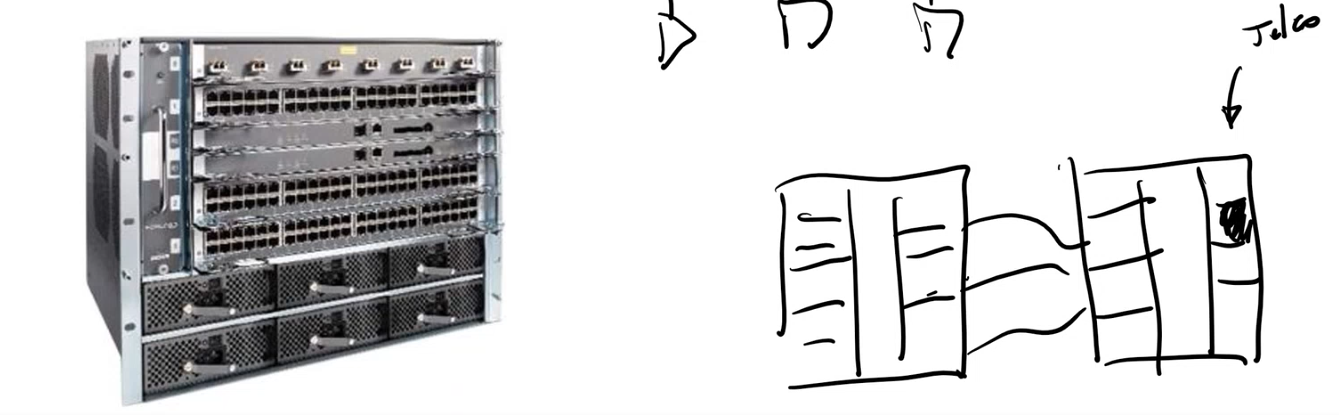
\includegraphics{images/network_chassis.png}
      \caption{Network chassis}
      \label{fig:network_chassis}
   \end{figure}

\end{paracol}
   
The Chassis is costful since it is a complex modular structure, so people tried to manage a stack of switches using protocols, making them act as if they a chassis.
The chassis provided redundancy for every component, and included ---two \smiley --- RPMs, routing processing modules.

Ports were numbered using $\langle line , port\rangle$. The line number was used to identify the line card, and the port number was used to identify the port on the line card. According to Cisternino this is important, and there is a ``lot of legacy''.

Chassis died when moving from 10Gbit/s to 25 and upper, because it was impossible to design a chassis the could allow hot replacing and modularity, and at the same time allow high speed links.
The size of the lanes and the type of the connector would limit the bandwidth and the frequency the physical link can resist.

Nowdays star solutions are rare to find. Starting from 2013/2014 it was not convenient to use chassis anymore, because they would get old too soon.
Swtiches started to have a fixed standard \textit{non-modular} form factor.\\
All vendors embedded proprietary protocols inside switches to allow to manage two switches as if they were one, and to aggregate two ports (one port for each switch) to have a single logical link, called \textbf{port channel}.
The standard protocol to do so, is called LACP (Link Aggregation Control Protocol) and is described in \ref{sec:LACP}.
\note{The port channel is a single logical link, but the bandwidth is \textit{not aggregated for the same data stream}.
However, the logical link provides redundancy and avoids loops.}

\subsection{Three-tier architecture}
\begin{paracol}{2}
   
   Simple architecture consisting of\ns
   \begin{enumerate}
      \item Core switches
      \item Aggregation switches
      \item Access switches
   \end{enumerate}\ns
   The switches are connected in a tree-like topology, with the core switches at the top, the aggregation switches in the middle, and the access switches at the bottom.\\
   STP is used to prevent loops in the network.

   Also provides active-passive redundancy which leads to inefficient east west traffic, because the traffic is forced to go through the core switches (?), and devices connected to the same port may contend for bandwidth.\\
   Moreover communication server-to-server might requires crossing between layer, causing latency and the abovementioned traffic bottleneck.
   
   \switchcolumn
   
   \colfill
   \begin{figure}[htbp]
      \centering
      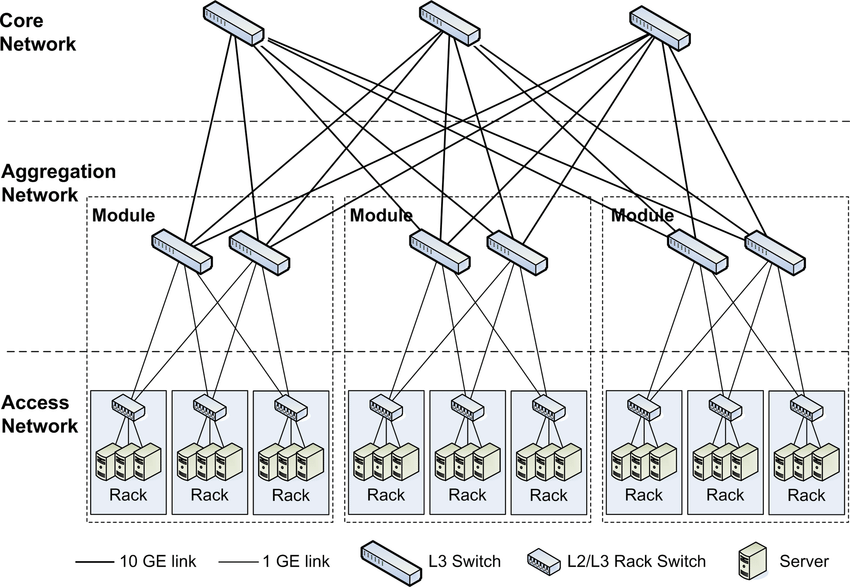
\includegraphics{images/3tier_switches.png}
      \caption{Three-tier architecture schema}
      \label{fig:3tier_switches}
   \end{figure}
   \colfill
   
\end{paracol}
This architecture is not used anymore, because it is not scalable, and it is not able to handle the high number of links and switches typical of a datacenter; more specifically, it does not fit virtualization most crucial need to be able to freely move VMs between servers.

\subsection{Spine Leaf architecture}
\begin{figure}[htbp]
   \centering
   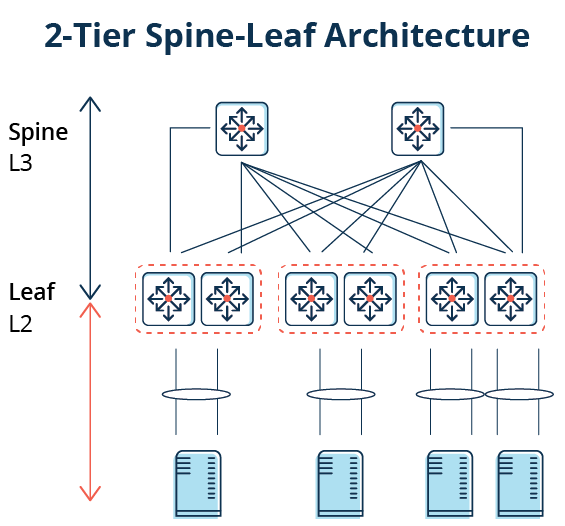
\includegraphics{images/spineleaf.png}
   \caption{Spine-leaf architecture schema (from \href{https://www.arubanetworks.com/faq/what-is-spine-leaf-architecture/}{Arubanetworks.com})}
   \label{fig:}
\end{figure}
A \textbf{spine-leaf} architecture is data center network topology that consists of two switching layers:
\begin{enumerate}
   \item \textbf{Spine layer}\\
   Swtiches responsible for routing traffic, working as the backbone of the network.   
   \item \textbf{Leaf layer}\\
   Switches connected to endpoints, such as servers, storage devices, firewalls, load balancers, edge routers, etc.
\end{enumerate}
Since \ul{every leaf switch is connected to every spine switch}, the spine-leaf architecture is a \textbf{fully connected} network,
ensuring that any source is always the same number of hops (actually only two or four \smiley) away from any destination, so latency is lower and predictable (fixed).

\note{
   ``However, it's not true that every rack is connected with any other rack.
   There is some topology that has been designed with the data center and it will.'' -Cisternino
}
Capacity also improves because STP is no longer required. While STP enables redundant paths between two switches, only one can be active at any time. As a result, paths often become oversubscribed. 
Conversely, spine-leaf architectures rely on protocols such as \textit{Equal-Cost Multipath} (\texttt{ECMP}) routing to load balance traffic across all available paths while still preventing network loops.

Spine-leaf allows \textit{scale-out} opposed to \textit{scale-up}, by adding additional spine switches, ultimately increasing capacity in case the bandwidth is not enough; doing so reduces also the subscription

\subsubsection{LACP}
\label{sec:LACP}
Loops are prevented using \texttt{LACP} (\textit{Link Aggregation Control Protocol}), which is a protocol that allows to aggregate multiple links into a single logical link, providing higher bandwidth and active-active redundancy (in case a link fails);
it also ensures no loops because each link is a single channel, and these are named \textit{port channels}.

LACP also provides a method to control the bundling of several physical ports together to form a single logical channel.

Note that even though the bandwidth is aggregated (i.e. $2\times 25Gbps$), the single stream is still limited to the bandwidth of a single link (i.e. $25Gbps$), because the traffic goes only from one way to the other each time.

\subsubsection{Advantages of Spine-Leaf}

\begin{itemize}
   \item Modular: you can mix and match devices with fixed size switches.
   \item Latency predictable: every host is distance one or two hops to each other host.
   \note{Actually it is 2 or 4 hops, because we have either\ns
   \begin{itemize}
      \item server $\rightarrow$ leaf, leaf $\rightarrow$ server
      \item server $\rightarrow$ leaf, leaf $\rightarrow$ spine, spine $\rightarrow$ leaf, leaf $\rightarrow$ server
   \end{itemize}
   However, the hops from server to leaf and viceversa are typically not counted as ``hops''.}
   \item Bandwidth control: it's possible to chose the proportion of NS and EW traffic and overbooking.
   \item Active-active redundancy:  both links of the port channels are enabled, so is the LACP to decide.
   \item Loop aware topology: a tree topology with no links disabled for redundancy reasons.
   \item Interconnect using standard cables (decide how many links use to interconnect spines with leaves and how many others link to racks).
   
\end{itemize}
With this architecture it’s possible to turn off one ---spine?--- switch, upgrade it and reboot it without compromising the network. Half of the bandwidth is lost in the process, but the twin\footnote{What does twin mean? Another spine?} switch keeps the connection alive.

Just a small remark: with spine and leaf we introduce \textbf{more hops}, so more latency, than the chassis approach, which basically represents a star topology, with the big network chassis as the center of the star. 
The solution for this problem is using as a base of the spine a huge switch (256 ports) which actually acts as a chassis, in order to reduce the number of hops and latency.

\subsubsection{Oversubscription}
Oversubscription is the practice of connecting multiple devices to the same
switch port to optimize the use. For example, it is particulary useful to connect multiple slower devices to a single port to take advantage of the unused
capacity of the port and improve its utilization. However, devices and applications that require high bandwidth should generally connect with a switch
port 1-on-1, because multiple devices connected to the same switch port may
contend for that port’s bandwidth, resulting in poor response time. Hence,
significant increases in the use of multi-core CPUs, server virtualization, flash
storage, Big Data and cloud computing have driven the requirement for modern networks to have lower oversubscription. For this reason, it is important
to keep in mind the oversubscription ratio (downlink ports ---to servers/storage--- to uplink ports ---to spina switches---), when designing the fabric.
Current modern network designs have oversubscription ratios of 3:1 or less, meaning that bandwidth for NS traffic in $\dfrac{1}{3}$ of the bandwidth for EW traffic.

\newpage
\subsubsection{Uplink and Downlink ratio}
``Uplink'' and ``downlink'' refers to the direction of the link in the topology. It appears more clear with a picture.

The ratio between uplink and downlink ports is important because it determines the bandwidth available to the servers. Typically the desired ratio is 1/3 of bandwidth uplink and 2/3 downlink.
So, considering the following switch having 20 QSFP ports (\texttt{40Gbit/s}) and 4 QSFP28 ports (\texttt{100Gbit/s}), we have:
\begin{itemize}
   \item 800 Gbit/s downlink, exploiting 20 QSFP
   \item 400 Gbit/s uplink, exploiting 4 QSFP28
\end{itemize}

\note{Even though traffic is categorized as NS or EW, there is also the \textit{aggregation traffic}, due to MLAG 
}
\begin{figure}[htbp]
   \centering
   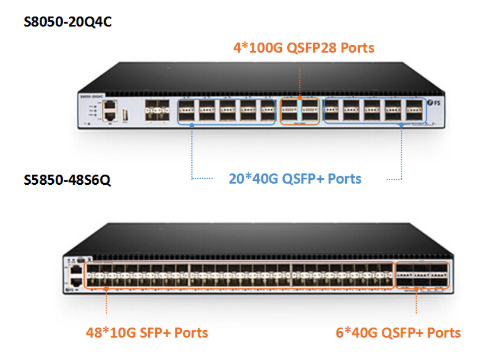
\includegraphics{images/downuplink_switch.png}
   \caption{Blue ports are downlink, yellow ports are uplink}
   \label{fig:downuplink_switch}
\end{figure}

\subsubsection{Considerations on Increasing Bandwidth}

In case the uplink bandwidth is not enough, it is possible to increase it by:
\begin{itemize}
   \item  adding more spine switches, and connecting them to the leaf switches.
   \begin{itemize}
      \item More redundancy in the paths between leaves, allowing to have even paths to the same destination
      \item More uplink ports needed, reducing oversubscription ratio
   \end{itemize}
   \item adding leaf switches, and redistributing the servers among them.
   \begin{itemize}
      \item Less downlink ports used per switch, reducing oversubscription ratio
      \item \textit{¡ACHTUNG!} Spine switches may need to be upgraded to support more leaves
   \end{itemize}
   \item adding a \textit{super-spine}, enhancing the number of hops but allowing to handle a huge number of servers.
\end{itemize}
The \textit{super-spine} fits an ``extreme'' scenario: the number of ports in spines is insufficient to handle the number of leaves.\\
Let's make a few calculations:
Considering that LACP allows to aggregate a maximum of 8 ports, but it is very unlikely to aggregate 8 ports from spines to leaves, since it would mean that every leaf switch has 8 ports for each spine.\\
Assuming to have respectively as spine and leaves the switches in Fig \ref{fig:downuplink_switch} and the oversubscription ratio to be 1:2, the maximum number of spines would be 6, and the maximum number of leaves 20.
Each leaf has 48 downlink ports, which however may be aggregated in 12 groups of 4 ports, hence 12 servers per leaf.\\
Summing up:
\begin{itemize}
   \item 6 spines
   \item 20 leaves per spine
   \item 12 servers (at least) per leaf
   \item $20 \times 12 = \textbf{240}$ servers units.
\end{itemize}
UniPi datacenter has 62 physical nodes, just for comparison.
Even assuming to halve the number of spines and to aggregate every pair of links from spines to leaves, the number of servers would be 240, still a pretty big number.

\framedt{How can a leaf know which is the best path to send its data onto?}{
   We want the path which is, at the moment of transmission, less used by other leaves and with more available bandwidth.\nl
   \note{Answered by Copilot \smiley}

   In a spine-and-leaf architecture, the decision on the best path for data transmission is typically made using routing protocols such as Equal-Cost Multipath (ECMP).

   ECMP is a routing strategy that allows traffic to be distributed across multiple paths of equal cost. This helps to balance the load across the network and utilize all available bandwidth. When a leaf switch has data to send, it uses ECMP to determine the best path among the multiple paths available.
   
   The decision is based on various factors such as the number of hops, path cost, and current network congestion. ECMP can dynamically adjust the traffic distribution based on the network conditions, ensuring that the data is always sent on the optimal path.
   
   So, in a spine-and-leaf architecture, the leaf switches don’t need to know the specific usage of other leaves. They rely on ECMP to determine the best path for data transmission. This allows the architecture to efficiently handle traffic and provide high performance, even in the presence of heavy east-west traffic.
}

\subsection{Full fat tree}
\begin{figure}[htbp]
   \centering
   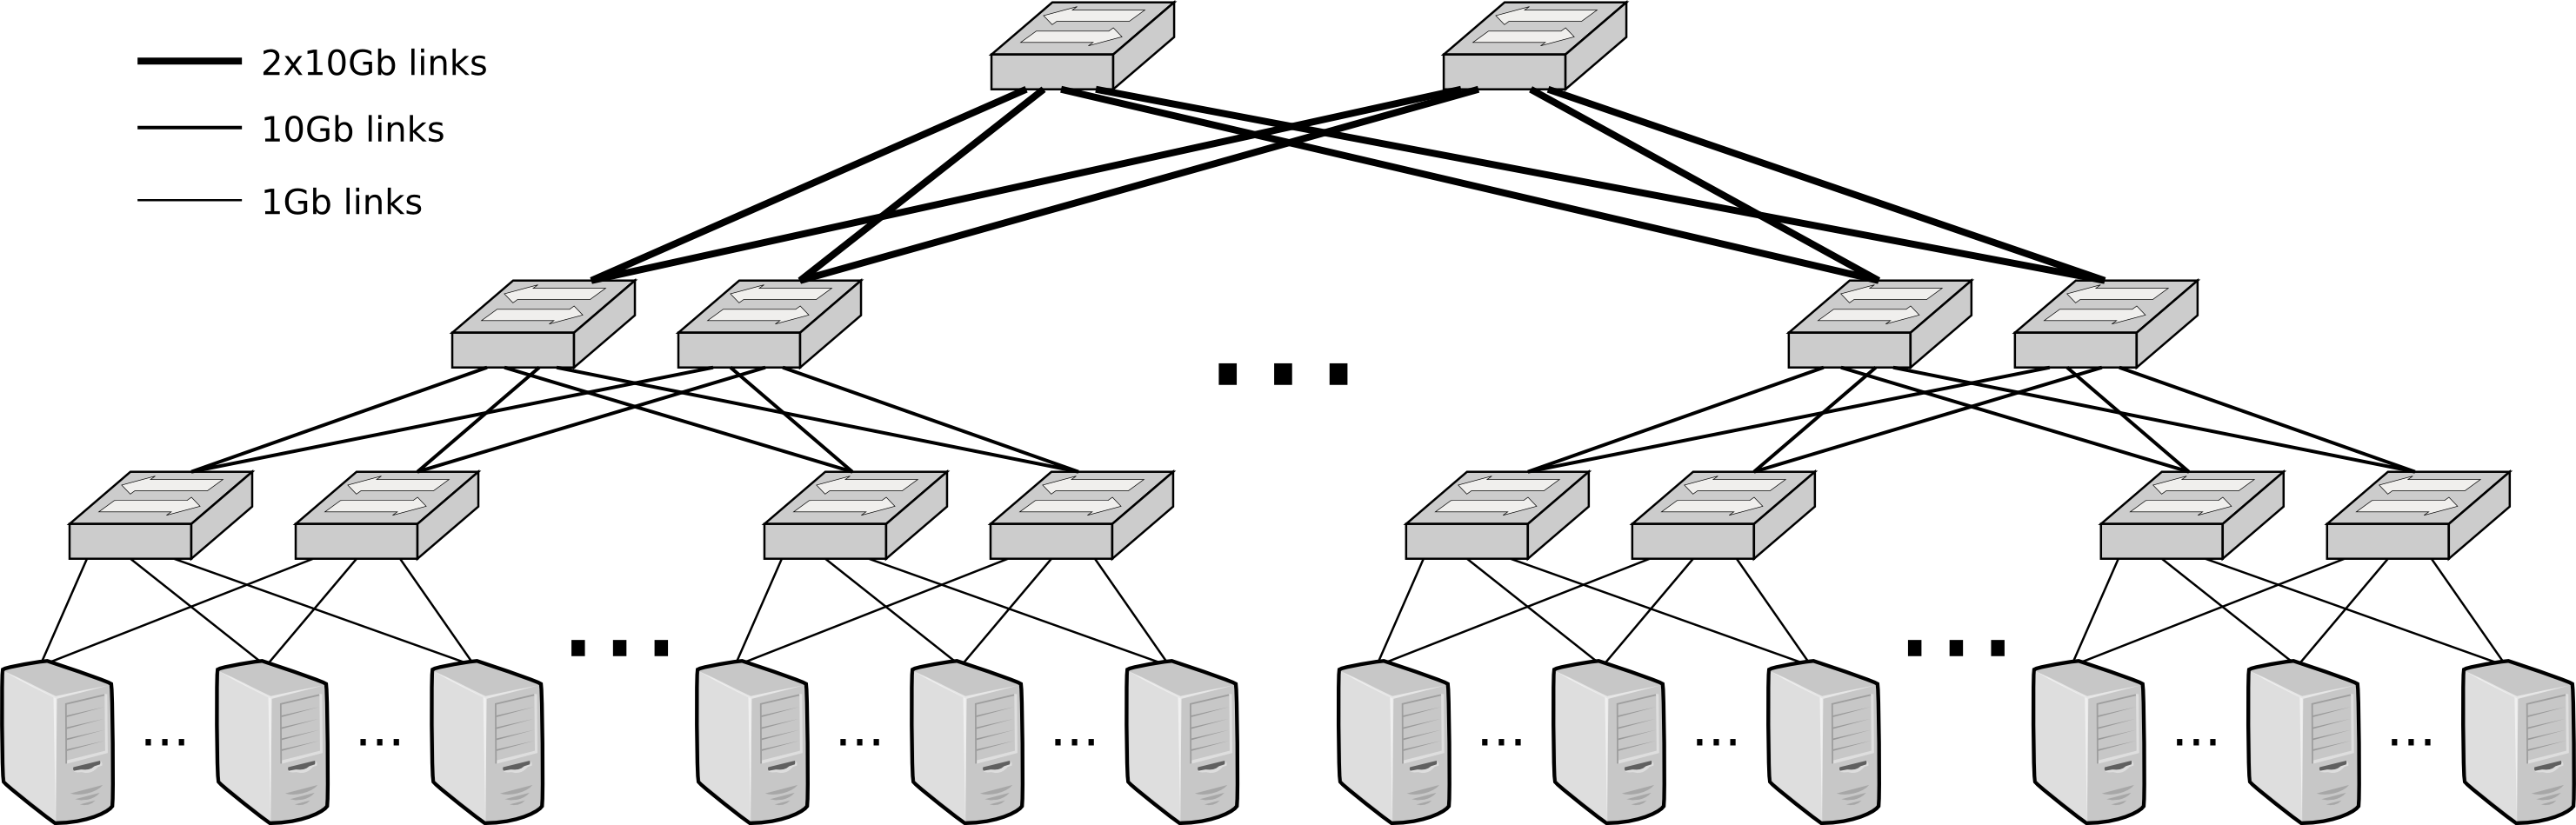
\includegraphics{images/fullfattree_network.png}
   \caption{Full fat tree network topology schema}
   \label{fig:fullfattree_network}
\end{figure}
In a \textbf{full fat tree} topology, branches nearer the top of the hierarchy are "fatter" (thicker) than branches further down the hierarchy. In a telecommunications network, the branches are data links; the varied thickness (bandwidth) of the data links allows for more efficient and technology-specific use, a typical use case is for HPC.
\note{Full-fat tree is rarely needed.}

The full fat tree resolves the problem of over-subscription. Adopting
the spine and leaf there is the risk that the links closer to the spines can’t sustain the traffic coming from all the links going from the servers to the leaves. The full fat tree is a way to build a tree so that the capacity is never
less than the incoming traffic. Since it's quite expensive some oversubscription can be accepted.

\begin{definition}[Full Fat Tree]
   ``The full fat tree is simply a spine and leaf architecture in which the bandwidth that you reserve to East West traffic is equivalent to the bandwidth that you reserve between the North and South uh traffic.''

   Hence, the oversubscription ratio is 1:1.
\end{definition}

\section{Virtualization}

\framedt{
   What's the key difference between Layer 2 and Layer 3?
}{
   There is \ul{no routing in layer 2}, \ul{\textbf{broadcast} is the standard way of communicating}.
   Potentially anyone who is physically in the same LAN can see the traffic of almost anyone else, slightly depending on the fabric.\\
   But luckily, \textbf{VLANs} exist. 
}

\begin{figure}[htbp]
   \centering
   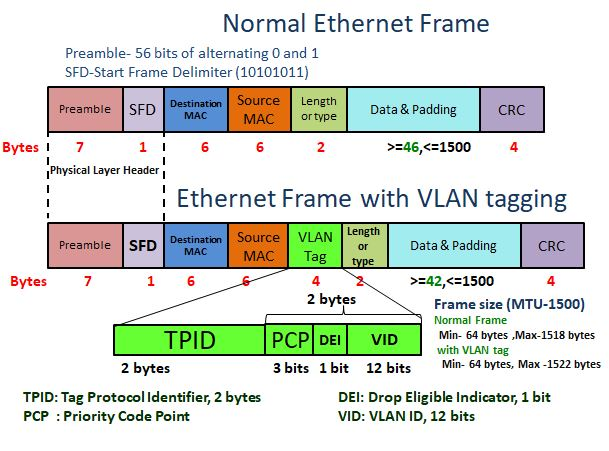
\includegraphics{images/vlan_header.jpg}
   \caption{Ethernet frame with VLAN header}
   \label{fig:vlan_header}
\end{figure}

With VLAN frames are extended by 4 bytes\footnote{12 bits are reserved for the VLAN ID allowing up to $4094$ ($4096-2$) logical partitions}. Every switch nowdays automatically sets the \texttt{VLAN\_ID} to \texttt{1}; if the field is not existent, it is appended, making an \textbf{untagged} a \textit{tagged} frame.

\ul{\textbf{Switches} ensure that data cannot spill/leak from a VLAN to another}, because they avoid sending traffic on ports which are not associated to the current VLAN.
VLAN became largely of use when 10Gbit connection came out, because only 1Gbit was a too constrained bandwidth to be splitted into multiple VLANs. 

VLAN are used to partition the traffic at data link layer without having to redo the fabric. They are particularly useful in cloud environments.

A port can be in three states (CISCO Terminology):\ns
\begin{itemize}
   

   \item \textbf{Access Mode}: An access port can have only one VLAN configured on the interface; it can carry traffic for only one VLAN1. It connects an end device to the network and works only in a single VLAN3.

   \item \textbf{Trunk Mode}: A trunk port can have two or more VLANs configured on the interface; it can carry traffic for several VLANs simultaneously1. Trunk mode is designed for connecting devices using tagged VLANs (e.g., VLAN-enabled switches and NICs). Ports using trunk mode can be linked between various network devices and are capable of carrying traffic across multiple VLANs4.

   \item \textbf{General Mode}: General mode allows multiple untagged VLANs and also multiple tagged VLANs to exist on the same switch interface2. While it is possible to have multiple untagged VLANs on a General port, you can only have ONE (1) PVID (Primary VLAN Identifier). The PVID represents the native VLAN. Untagged traffic may be sent via several untagged VLANs, returning untagged traffic will only be received by the PVID and therefore will NOT be forwarded to a specific VLAN2.

   \end{itemize}

\section{Network Administrator POV}
The switch is split in two planes:
\begin{itemize}
   \item \textbf{Control Plane}\\
   This plane is necessary to configure the data plane to make it behave according to our needs.
   Here there is an \textit{OS}, which used to be proprietary with a functioning fitting a specific network configuration, but nowdays they are usually more configurable and may even be \textit{open} OS.
   \note{\textit{Dell}'s switches now have an \textit{open} OS on board.}
   
   \item \textbf{Data Plane}\\
   Here lies the chip responsible to perform all the data link operations required, runs protocols, handles VLANs, etc.

   \textbf{OpenFlow} allows us to manage the flow table inside of a switch.
\end{itemize}

The two planes are linked by a low-bandwidth PCIe.


It is possible to use a very fast and simple ---reduced number of keystroke down to the strict necessary ones (e.g. \texttt{en} instead of \texttt{enable})--- CLI to program a switch. It is also possible to create a script file to be automatically executed by the switch at boot time.
\note{Prof. Cisternino performed a demo of this in class.}

Interestingly, the behaviour of the \texttt{netsh} command in Windows is very similar to the one of a switch.
